\documentclass[a4paper,11pt,UTF8]{article}
\usepackage{ctex}
\usepackage{amsmath,amsthm,amssymb,amsfonts}
\usepackage{amsmath}
\usepackage[a4paper]{geometry}
\usepackage{graphicx}
\usepackage{microtype}
\usepackage{siunitx}
\usepackage{booktabs}
\usepackage[colorlinks=false, pdfborder={0 0 0}]{hyperref}
\usepackage{cleveref}
\usepackage{esint} 
\usepackage{graphicx}
\usepackage{ragged2e}
\usepackage{pifont}
\usepackage{extarrows}
\usepackage{mathptmx}
\usepackage{float}
\usepackage{caption}
\usepackage{multirow}
\usepackage{subfigure}
\usepackage{titlesec}
\captionsetup[figure]{name={图}}
%opening
\title{数字电子技术作业(四)}
\author{谢悦晋 \quad U202210333}
\date{Nov 2nd, 2023 }
\begin{document}
\maketitle
\textbf{5.4.6} 由$D$触发器和数据选择器构成的电路,以及各个输入信号 $EN$ ,$A$ 和时钟脉冲 $CP$ 的波形如图题 5.4.6所示。试画出输出$Q_0$与$Q_1$的波形。设触发器的初始状态均为0。
\begin{figure}[H]
	\centering
	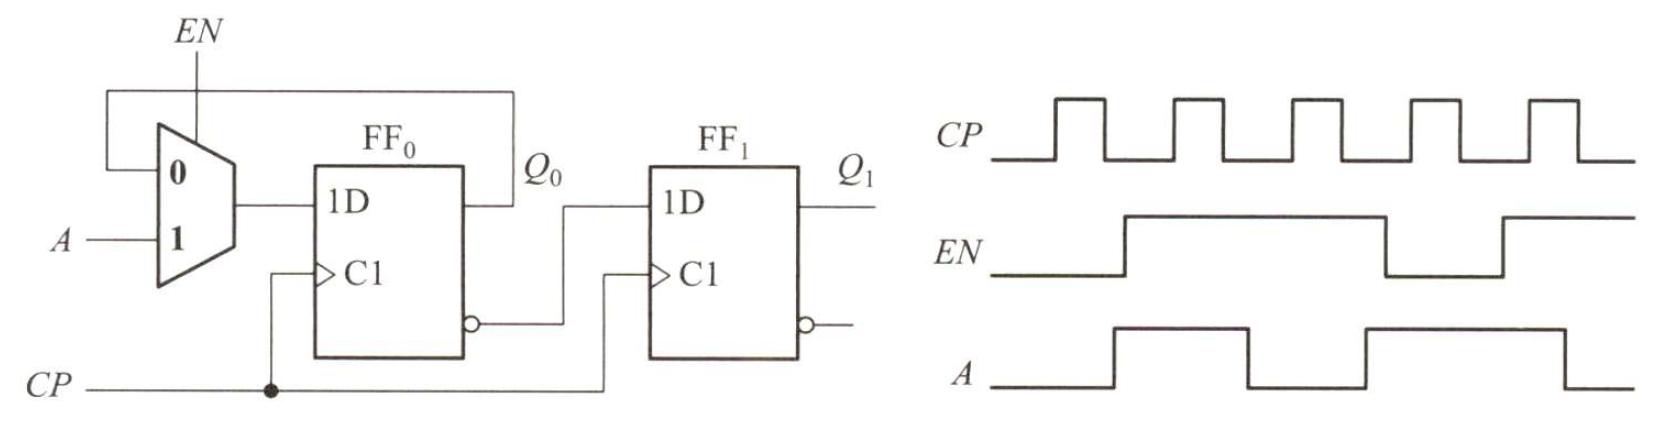
\includegraphics[width=0.9\textwidth]{5.4.6}
\end{figure}
解:波形如下:
\begin{figure}[H]
	\centering
	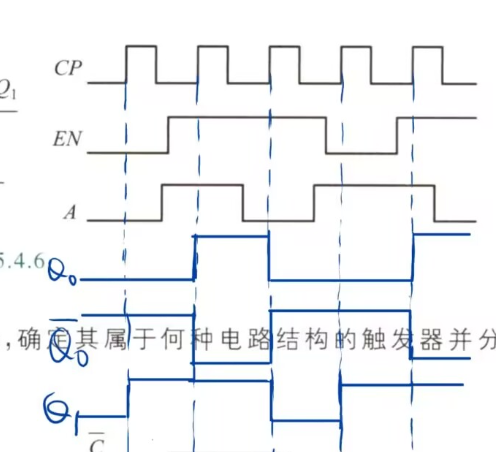
\includegraphics[width=0.9\textwidth]{5.4.6_1}
\end{figure}
\textbf{5.5.3} 逻辑电路和各输入信号波形如图题 5.5.3 所示,$R$ 为异步清零端。画出两触发器 $Q$ 端的波形。设触发器的初始状态均为0。
\begin{figure}[H]
	\centering
	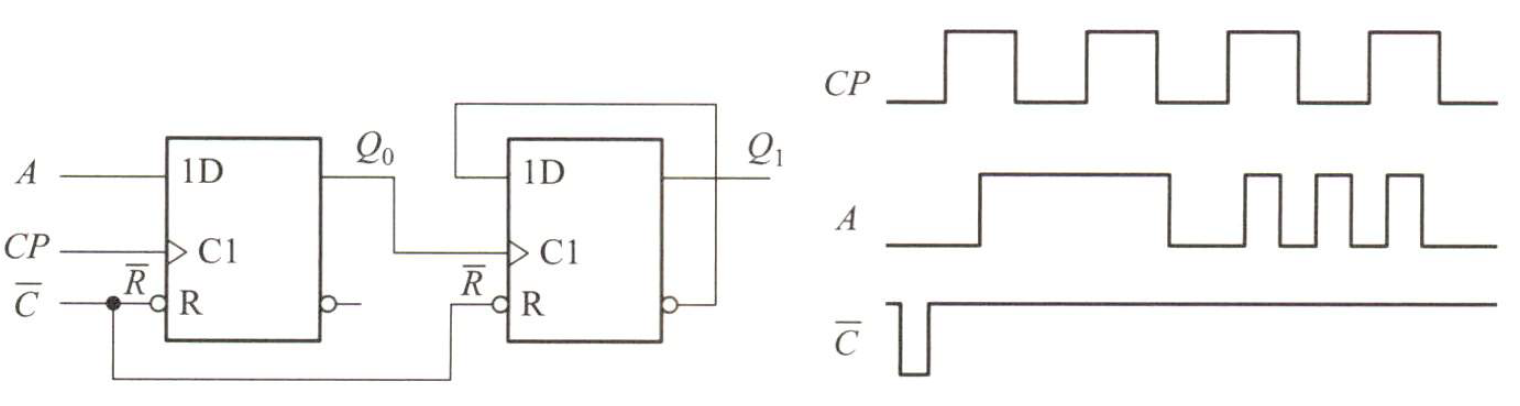
\includegraphics[width=0.9\textwidth]{5.5.3}
\end{figure}
解:波形如下:
\begin{figure}[H]
	\centering
	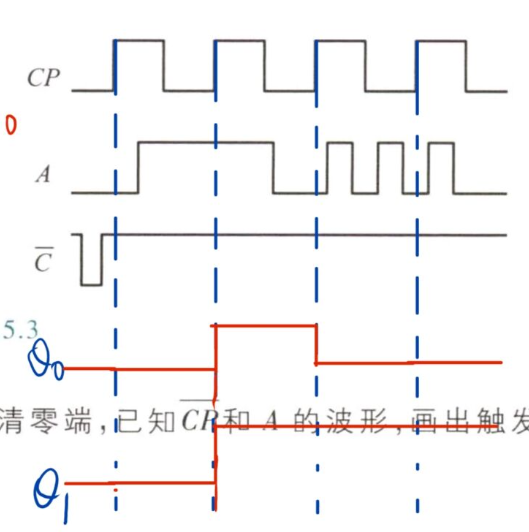
\includegraphics[width=0.9\textwidth]{5.5.3_1}
\end{figure}
\textbf{5.5.9} 逻辑电路如图题 5.5.9 所示,已知$\overline{CP}$和$X$ 的波形,试画出$Q_{\mathrm{o}}$和$Q_{\mathrm{i}}$的波形。触发器的初始状态均为 0。
\begin{figure}[H]
	\centering
	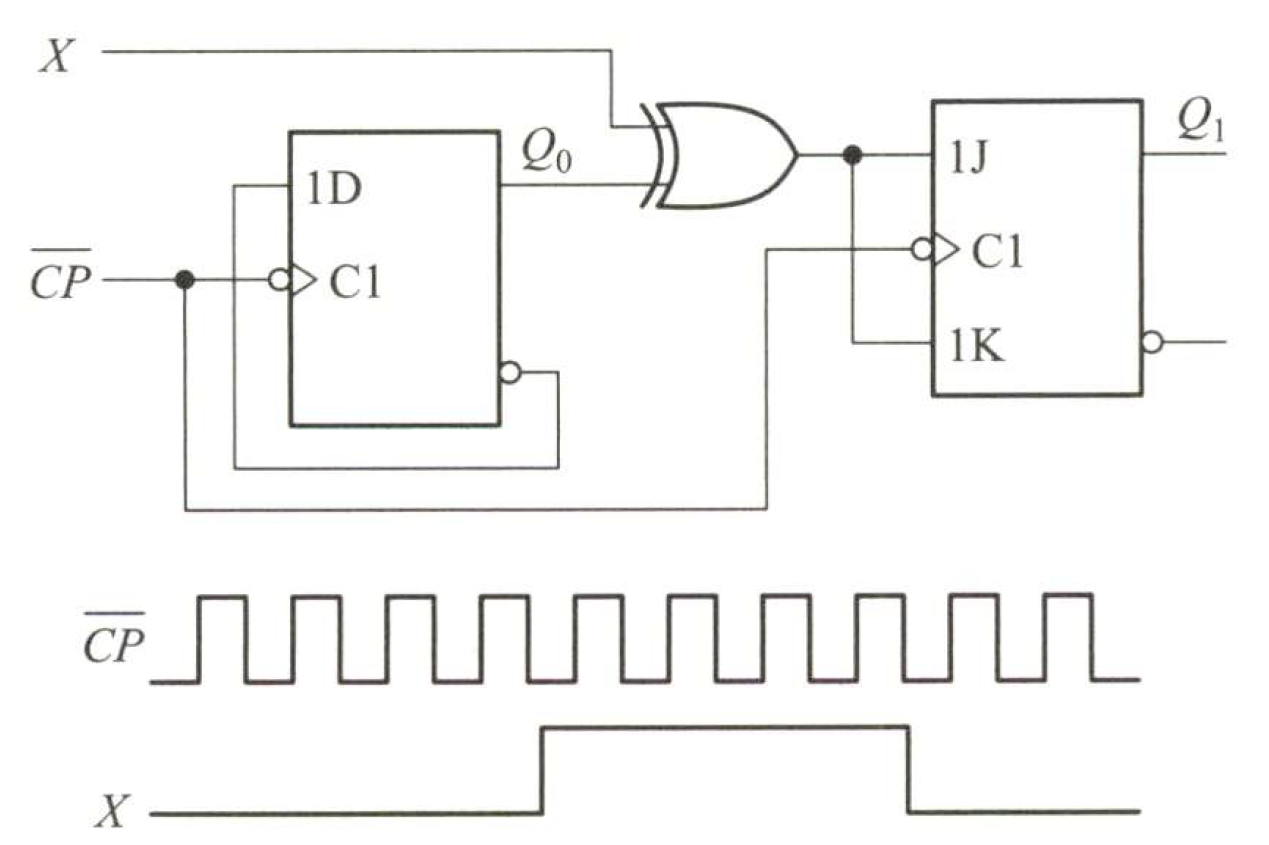
\includegraphics[width=0.7\textwidth]{5.5.9}
\end{figure}
解:波形如下:
\begin{figure}[H]
	\centering
	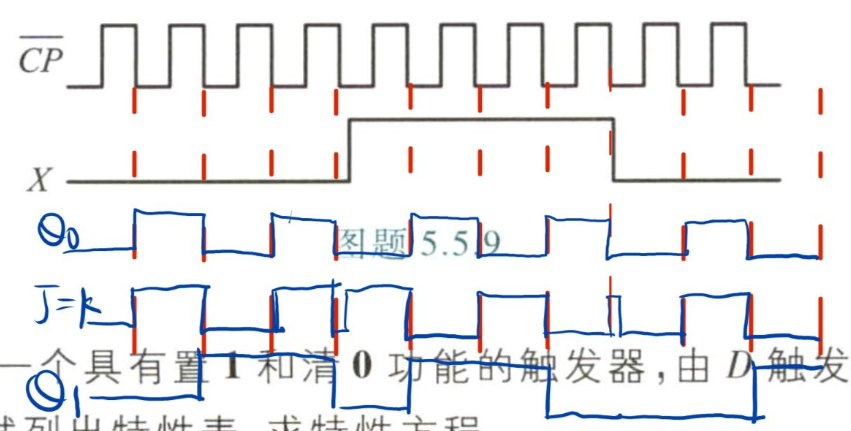
\includegraphics[width=0.9\textwidth]{5.5.9_1}
\end{figure}\newpage
波形整形电路: 由于敲击按键速度不同,X为高电平的时间长短不一。为避免后续电路的误动作,设计波形整形电路。当电路的输入X为高电平后,将在下一个时钟上升沿到来时,其输出信号Z将产生一个时钟周期的高电平,Z在其他时间为低电平。
\begin{figure}[H]
	\centering
	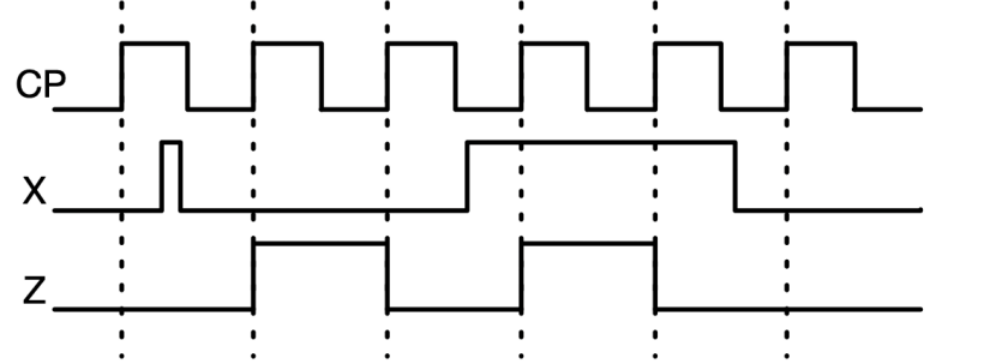
\includegraphics[width=0.7\textwidth]{5_class}
\end{figure}
电路设计的要点:(1)X与时钟异步,X为高电平的时间长短不重要;(2)两个D触发器,除了触发器的时钟,触发器的异步清零和异步置位信号灵活运用;(3)找到输入输出之间的关系,以搭积木方式进行电路设计
\end{document}